% !TeX spellcheck = de_DE
\documentclass[ngerman,12pt]{article}

% Packages for Language
\usepackage[ngerman]{babel}
\usepackage[utf8]{inputenc}
\usepackage[T1]{fontenc}
\usepackage[final]{graphicx}
\usepackage{amsmath}
\usepackage{float}
%\usepackage{wrapfig}
\usepackage{caption}
%\usepackage{multirow}
\usepackage{subfig}
\usepackage{hyperref}
\usepackage[german, plain]{fancyref}
\usepackage{afterpage,pdflscape} %%% !!!!!!! CHANGE TO PDFLSCAPE LATER!
\usepackage{varioref}
\usepackage{siunitx}
\usepackage{translator}
\usepackage{listings}
\usepackage{fancyhdr}
\pagestyle{fancy}

\setlength{\headheight}{15.5pt}
\lhead{NAME NAME NAME}
\rhead{\today}
\chead{Numerik Übung 6}


\begin{document}
\lstset{language=Matlab,basicstyle=\ttfamily,columns=fixed}
\subsubsection*{main.m}
\begin{lstlisting}[frame=single]
x = [-1.5;-1;0;1;0;-1;0;1;0;-1;0;1;0;-1;-1.5];
y = [0;0;-1;0;1;0;-1;0;1;0;-1;0;1;0;0];
z = [-6;-6;-5;-4;-3;-2;-1;0;1;2;3;4;5;6;6]./6;
t = getT(x,y,z);
Nx = divDiff(t, x);
Ny = divDiff(t, y);
Nz = divDiff(t, z);
tp = linspace(t(1), t(end), 666);
xp = hornerNewton(Nx, t, tp);
yp = hornerNewton(Ny, t, tp);
zp = hornerNewton(Nz, t, tp);
plot3(x, y, z, 'ks', xp, yp, zp, 'r-');
axis equal; view(-35, 40);
axis([-1.6, 1.1, -1.1, 1.1, -1.1, 1.1]);
\end{lstlisting}

\subsubsection*{divDiff.m}
\begin{lstlisting}[frame=single]
function [ N ] = divDiff( x, y )
n=length(y);
N=y;
for i=1:n-1
  N(i+1:n)=(N(i+1:n)-N(i:n-1))./(x(i+1:n)-x(1:n-i));
end
end
\end{lstlisting}
\filbreak
\subsubsection*{hornerNewton.m}
\begin{lstlisting}[frame=single]
function [ p ] = hornerNewton( N, x, xi )
n=length(N);
p=N(n)*ones(size(xi));
for i=n-1:-1:1
  p = p.*(xi-x(i))+N(i);
end
end
\end{lstlisting}

\subsubsection*{getT.m}
\begin{lstlisting}[frame=single]
function [ t ] = getT( x,y,z )
n=length(x);
t=zeros(size(x));
for i=2:n
  t(i)=t(i-1)+(x(i)-x(i-1)).^2 +...
    (y(i)-y(i-1)).^2 + (z(i)-z(i-1)).^2;
end
end
\end{lstlisting}

\subsubsection*{Output}
\begin{figure}[H]
    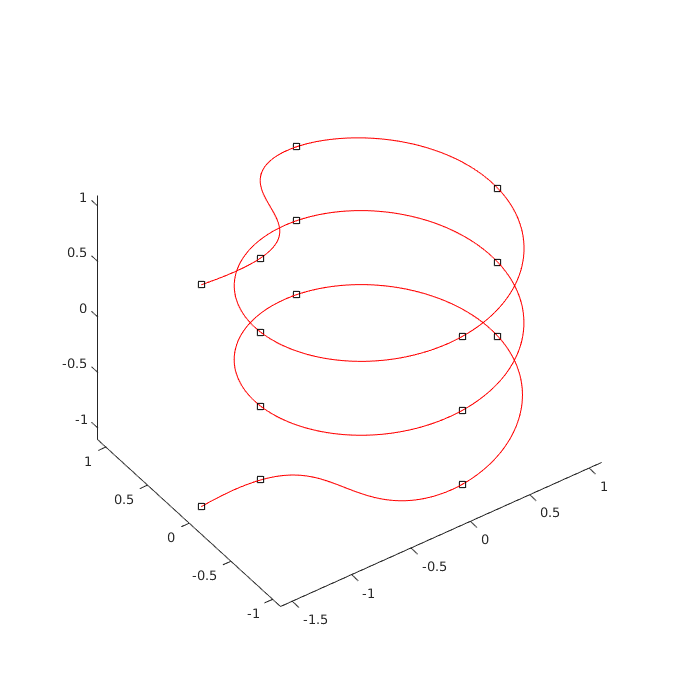
\includegraphics[width=0.88\linewidth]{m5.png}
\end{figure}

\end{document}